\documentclass[11pt]{article}

\usepackage{float}   % 👈必须加这个
\usepackage{graphicx}
\usepackage{amsmath}
\usepackage{booktabs}
\usepackage{geometry}
\geometry{margin=1in}

\title{Heart Failure Survival Prediction Using Machine Learning: A Clinical Data-Driven Analysis}
\author{Xueyan Weng}
\date{}

\begin{document}
	
	\maketitle
	
	% ==================================================
	\section{Abstract}
	% ==================================================
	
	Heart failure is a severe cardiovascular condition with high mortality risk. This study investigates survival prediction using clinical data from 299 patients and applies machine learning methods including Logistic Regression and Random Forest.
	
	Beyond prediction, this work focuses on interpretability and clinical consistency. We analyze feature distributions, inter-variable relationships, and model explanations to understand which clinical indicators contribute most to mortality risk.
	
	Results show that Random Forest achieves higher discriminative performance (AUC = 0.883) than Logistic Regression (AUC = 0.859). However, recall remains limited due to class imbalance. Serum creatinine, ejection fraction, and age are consistently identified as key risk factors.
	
	% ==================================================
	\section{Introduction}
	% ==================================================
	
	Heart failure is one of the leading causes of hospitalization and mortality worldwide. Early identification of high-risk patients is essential for timely intervention.
	
	Traditional clinical scoring systems rely heavily on linear assumptions and expert experience. However, patient physiology is often nonlinear and interactive in nature. Machine learning models can capture these complex relationships and improve predictive performance.
	
	This study aims not only to build predictive models but also to interpret clinical risk patterns from a data-driven perspective.
	
	% ==================================================
	\section{Dataset Overview and Statistical Characteristics}
	% ==================================================
	
	The dataset consists of 299 patients with 13 clinical variables, including demographic factors, laboratory measurements, and lifestyle indicators.
	
	The target variable is DEATH\_EVENT, indicating whether the patient died during the follow-up period.
	
	The overall mortality rate is 32.1\%, which introduces a moderate class imbalance problem.
	
	\begin{figure}[H]
		\centering
		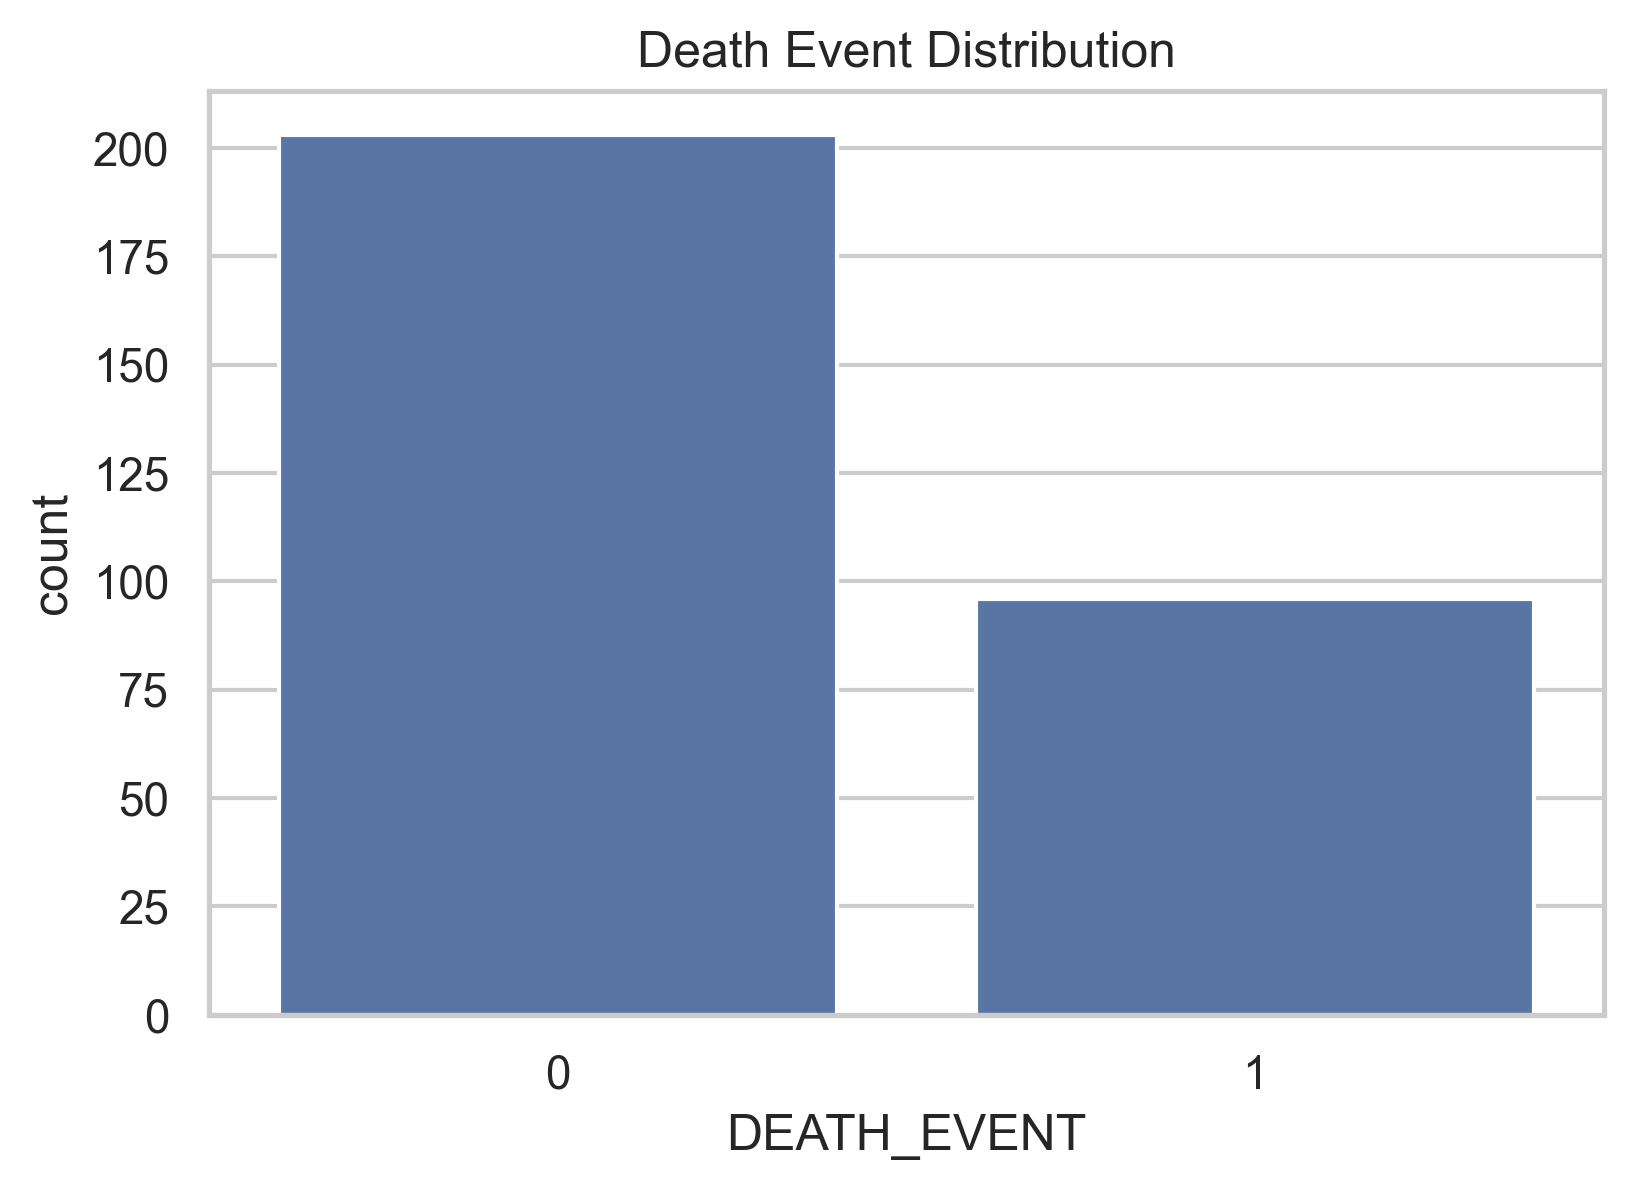
\includegraphics[width=0.6\textwidth]{../figures/death_distribution.png}
		\caption{Class distribution of survival and death cases}
	\end{figure}
	
	\subsection{Analysis of Class Imbalance}
	
	From the figure, it is evident that survival cases significantly outnumber death cases. This imbalance is critical for model behavior.
	
	In classification problems, models tend to be biased toward the majority class. As a result, although accuracy may remain high, recall for the minority class (death events) tends to decrease.
	
	This is clearly reflected in the results, where recall remains at approximately 0.58 for both models.
	
	Therefore, class imbalance is not merely a data property but a key factor affecting clinical reliability of predictive models.
	
	% ==================================================
	\section{Exploratory Feature Analysis}
	% ==================================================
	
	\subsection{Global Feature Correlation Structure}
	
	\begin{figure}[H]
		\centering
		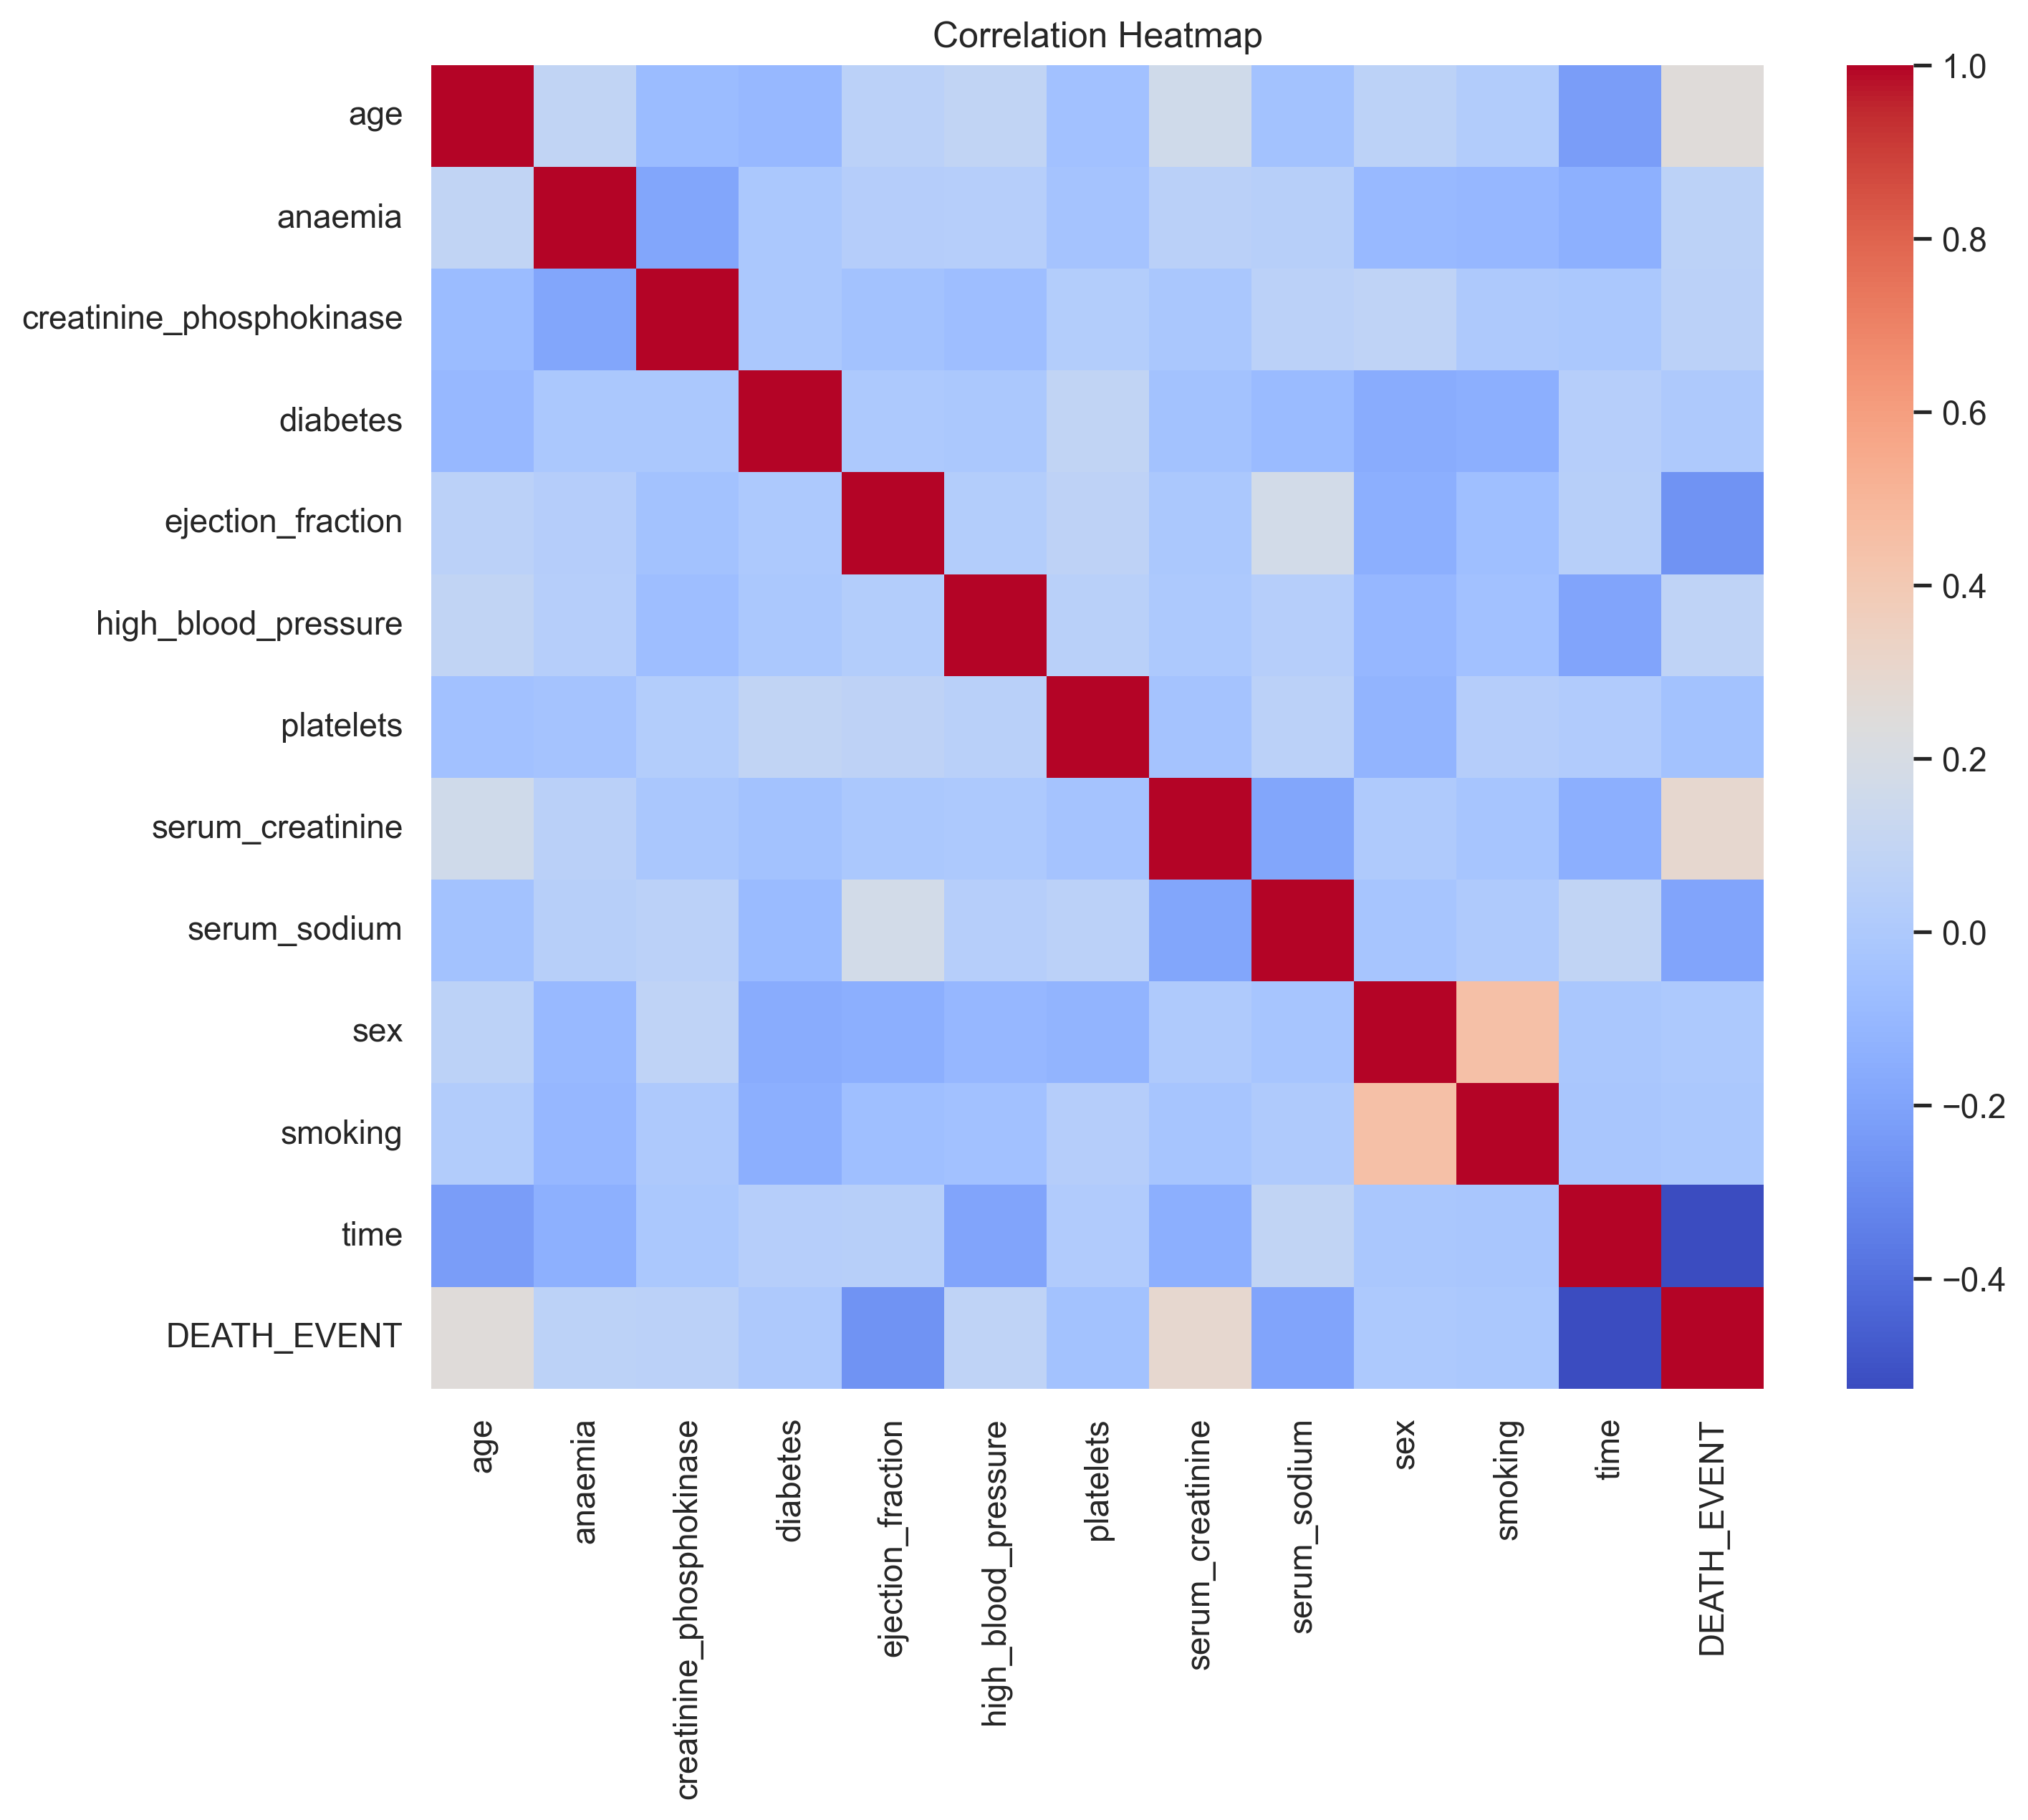
\includegraphics[width=0.8\textwidth]{../figures/correlation_heatmap.png}
		\caption{Correlation heatmap of clinical variables}
	\end{figure}
	
	The correlation heatmap provides a global view of relationships between variables.
	
	Two clinically meaningful patterns emerge:
	
	\begin{itemize}
		\item Ejection fraction is negatively correlated with mortality.
		\item Serum creatinine is positively correlated with mortality.
	\end{itemize}
	
	This indicates that cardiac function and renal function are the two most important physiological systems affecting survival.
	
	Interestingly, some variables such as smoking and diabetes show weak correlations. This does not necessarily mean they are unimportant; rather, their effects may be nonlinear or mediated by other variables.
	
	\subsection{Age as a Risk Factor}
	
	\begin{figure}[H]
		\centering
		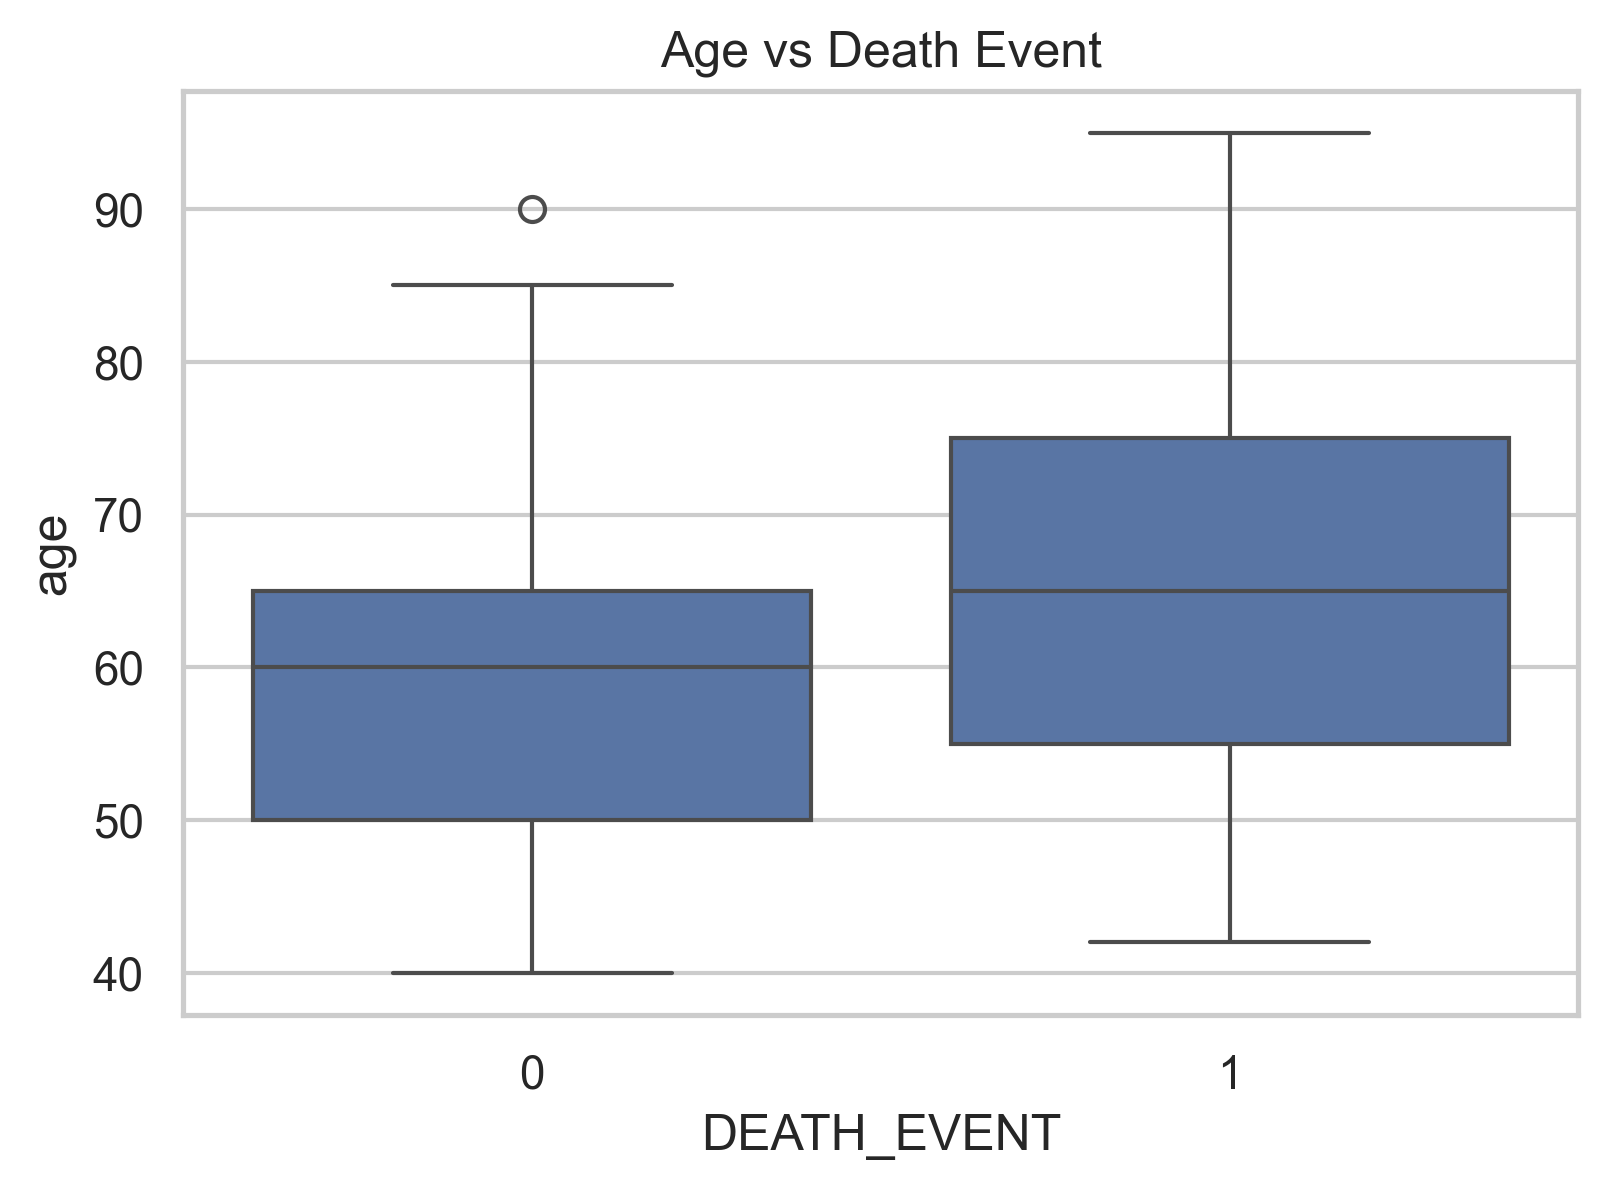
\includegraphics[width=0.6\textwidth]{../figures/age_vs_death.png}
		\caption{Age distribution in relation to mortality}
	\end{figure}
	
	Age shows a clear upward trend in mortality risk. However, the relationship is not strictly linear.
	
	Instead, mortality increases more sharply in older age groups (above ~65 years). This suggests that age may interact with other comorbidities rather than acting as an isolated predictor.
	
	From a clinical perspective, aging is associated with reduced cardiac reserve, increased vascular stiffness, and higher prevalence of chronic diseases, all contributing to worse outcomes.
	
	\subsection{Ejection Fraction: Cardiac Performance Indicator}
	
	\begin{figure}[H]
		\centering
		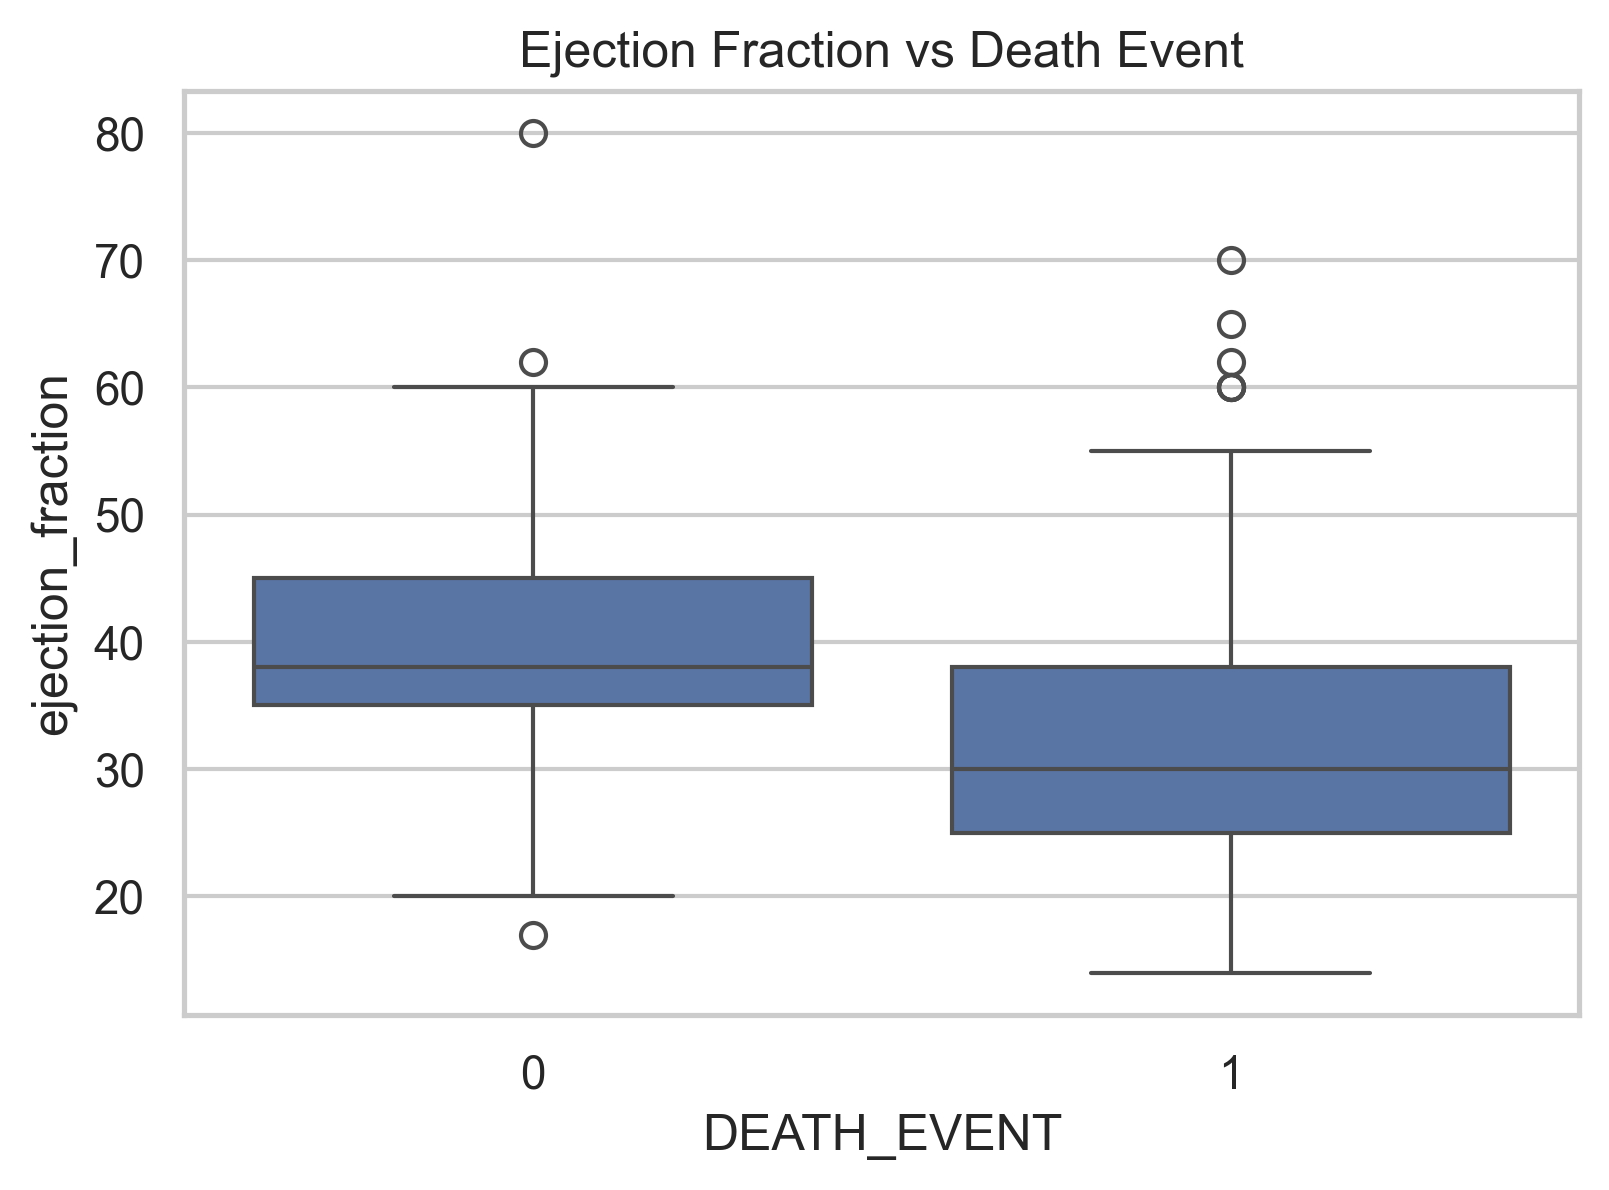
\includegraphics[width=0.6\textwidth]{../figures/ejection_fraction_vs_death.png}
		\caption{Ejection fraction vs mortality outcome}
	\end{figure}
	
	Ejection fraction (EF) is one of the strongest predictors observed in the dataset.
	
	Patients with low EF exhibit substantially higher mortality rates. This reflects reduced pumping efficiency of the heart.
	
	Importantly, the separation between survival and death groups becomes more pronounced at very low EF values, suggesting a threshold-like behavior rather than a smooth linear relationship.
	
	This nonlinear pattern justifies the use of tree-based models such as Random Forest.
	
	\subsection{Serum Creatinine and Renal Function}
	
	\begin{figure}[H]
		\centering
		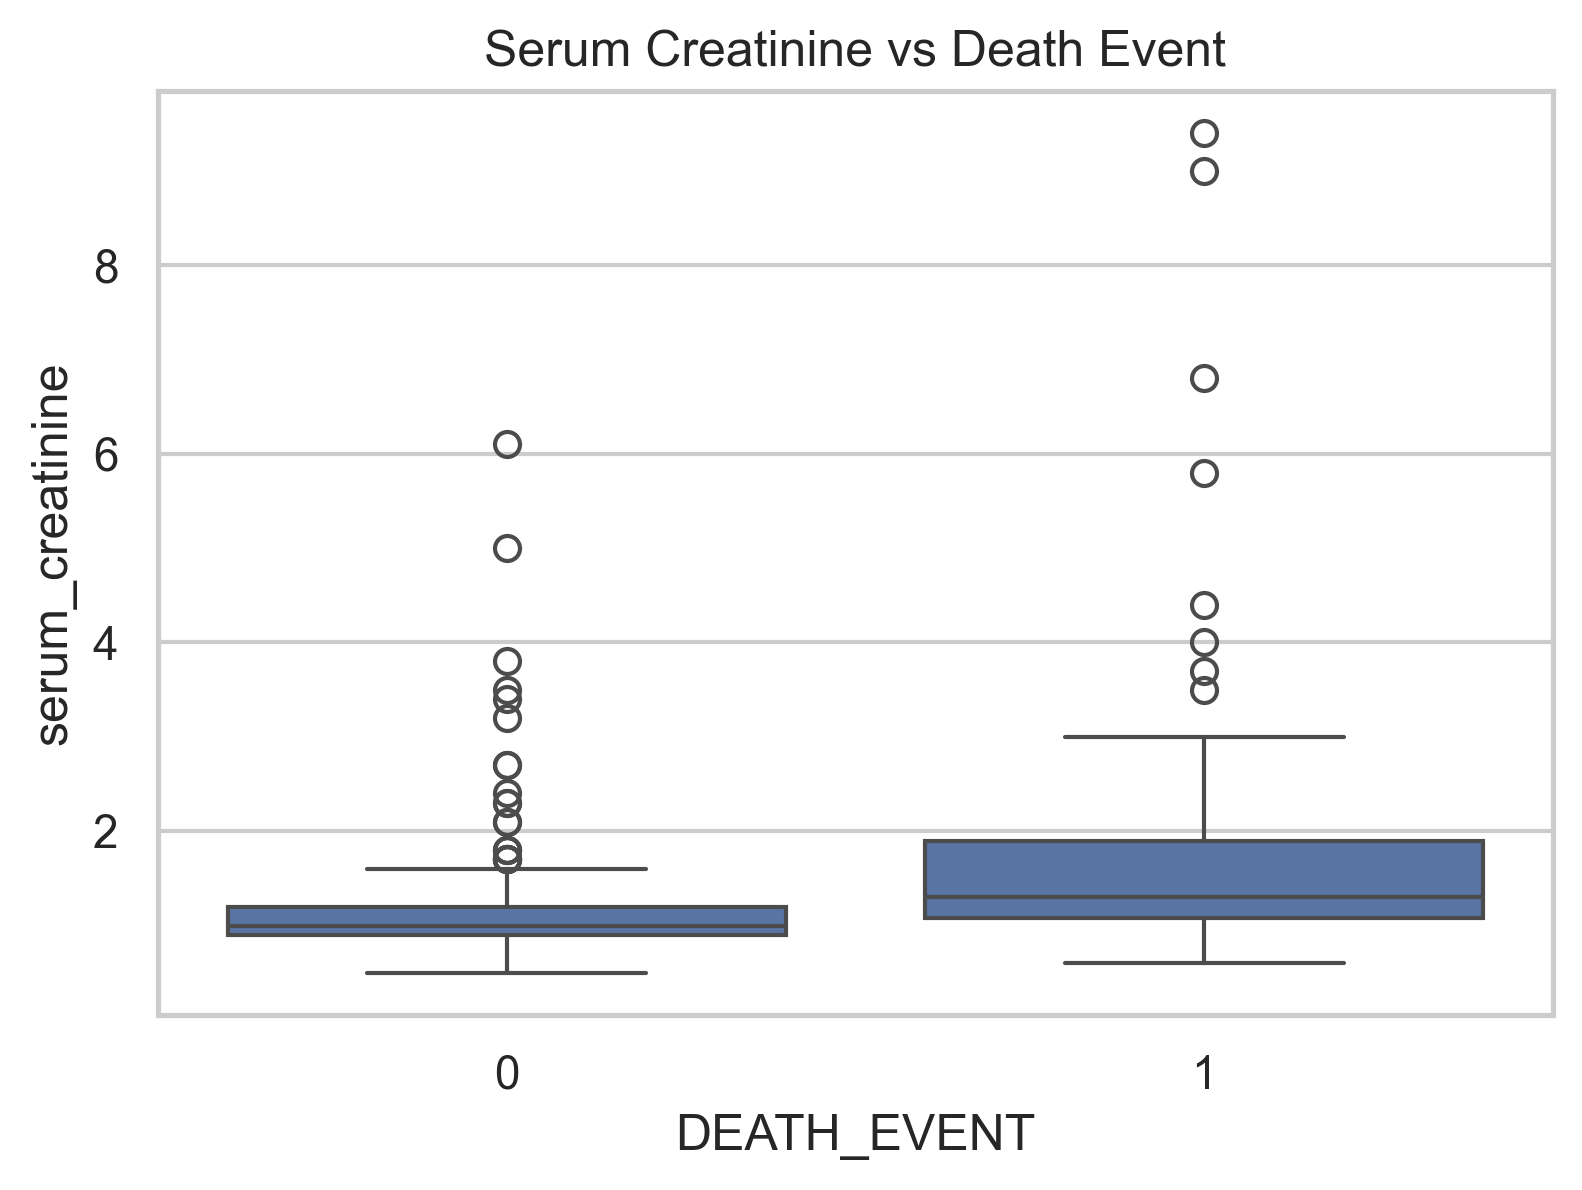
\includegraphics[width=0.6\textwidth]{../figures/serum_creatinine_vs_death.png}
		\caption{Serum creatinine levels vs mortality}
	\end{figure}
	
	Serum creatinine shows a strong positive association with mortality.
	
	Patients with higher creatinine levels are significantly more likely to experience death events. Clinically, this reflects impaired kidney function, which often coexists with heart failure.
	
	More importantly, the effect appears nonlinear: risk increases sharply beyond a certain threshold, indicating potential physiological decompensation.
	
	This further supports the need for nonlinear modeling approaches.
	
	% ==================================================
	\section{Machine Learning Methodology}
	% ==================================================
	
	Two models are employed:
	
	\begin{itemize}
		\item Logistic Regression: interpretable linear baseline model
		\item Random Forest: nonlinear ensemble learning model
	\end{itemize}
	
	The dataset is split into training (80\%) and testing (20\%) sets. Feature standardization is applied for Logistic Regression to ensure stable convergence.
	
	The F1-score is defined as:
	
	\begin{equation}
		F1 = 2 \cdot \frac{Precision \cdot Recall}{Precision + Recall}
	\end{equation}
	
	This metric is particularly important in imbalanced datasets, as it balances sensitivity and specificity.
	
	% ==================================================
	\section{Results and Model Evaluation}
	% ==================================================
	
	\subsection{Quantitative Performance}
	
	\begin{table}[H]
		\centering
		\begin{tabular}{lccccc}
			\toprule
			Model & Accuracy & Precision & Recall & F1-score & AUC \\
			\midrule
			Logistic Regression & 0.817 & 0.786 & 0.579 & 0.667 & 0.859 \\
			Random Forest & 0.817 & 0.786 & 0.579 & 0.667 & 0.883 \\
			\bottomrule
		\end{tabular}
		\caption{Comparison of model performance}
	\end{table}
	
	Although both models achieve identical accuracy and F1-score, Random Forest demonstrates superior AUC performance, indicating better ranking ability across different decision thresholds.
	
	However, both models exhibit relatively low recall. This is a critical limitation in medical prediction tasks, where failing to identify high-risk patients may have severe consequences.
	
	\subsection{Interpretation of Feature Importance}
	
	\begin{figure}[H]
		\centering
		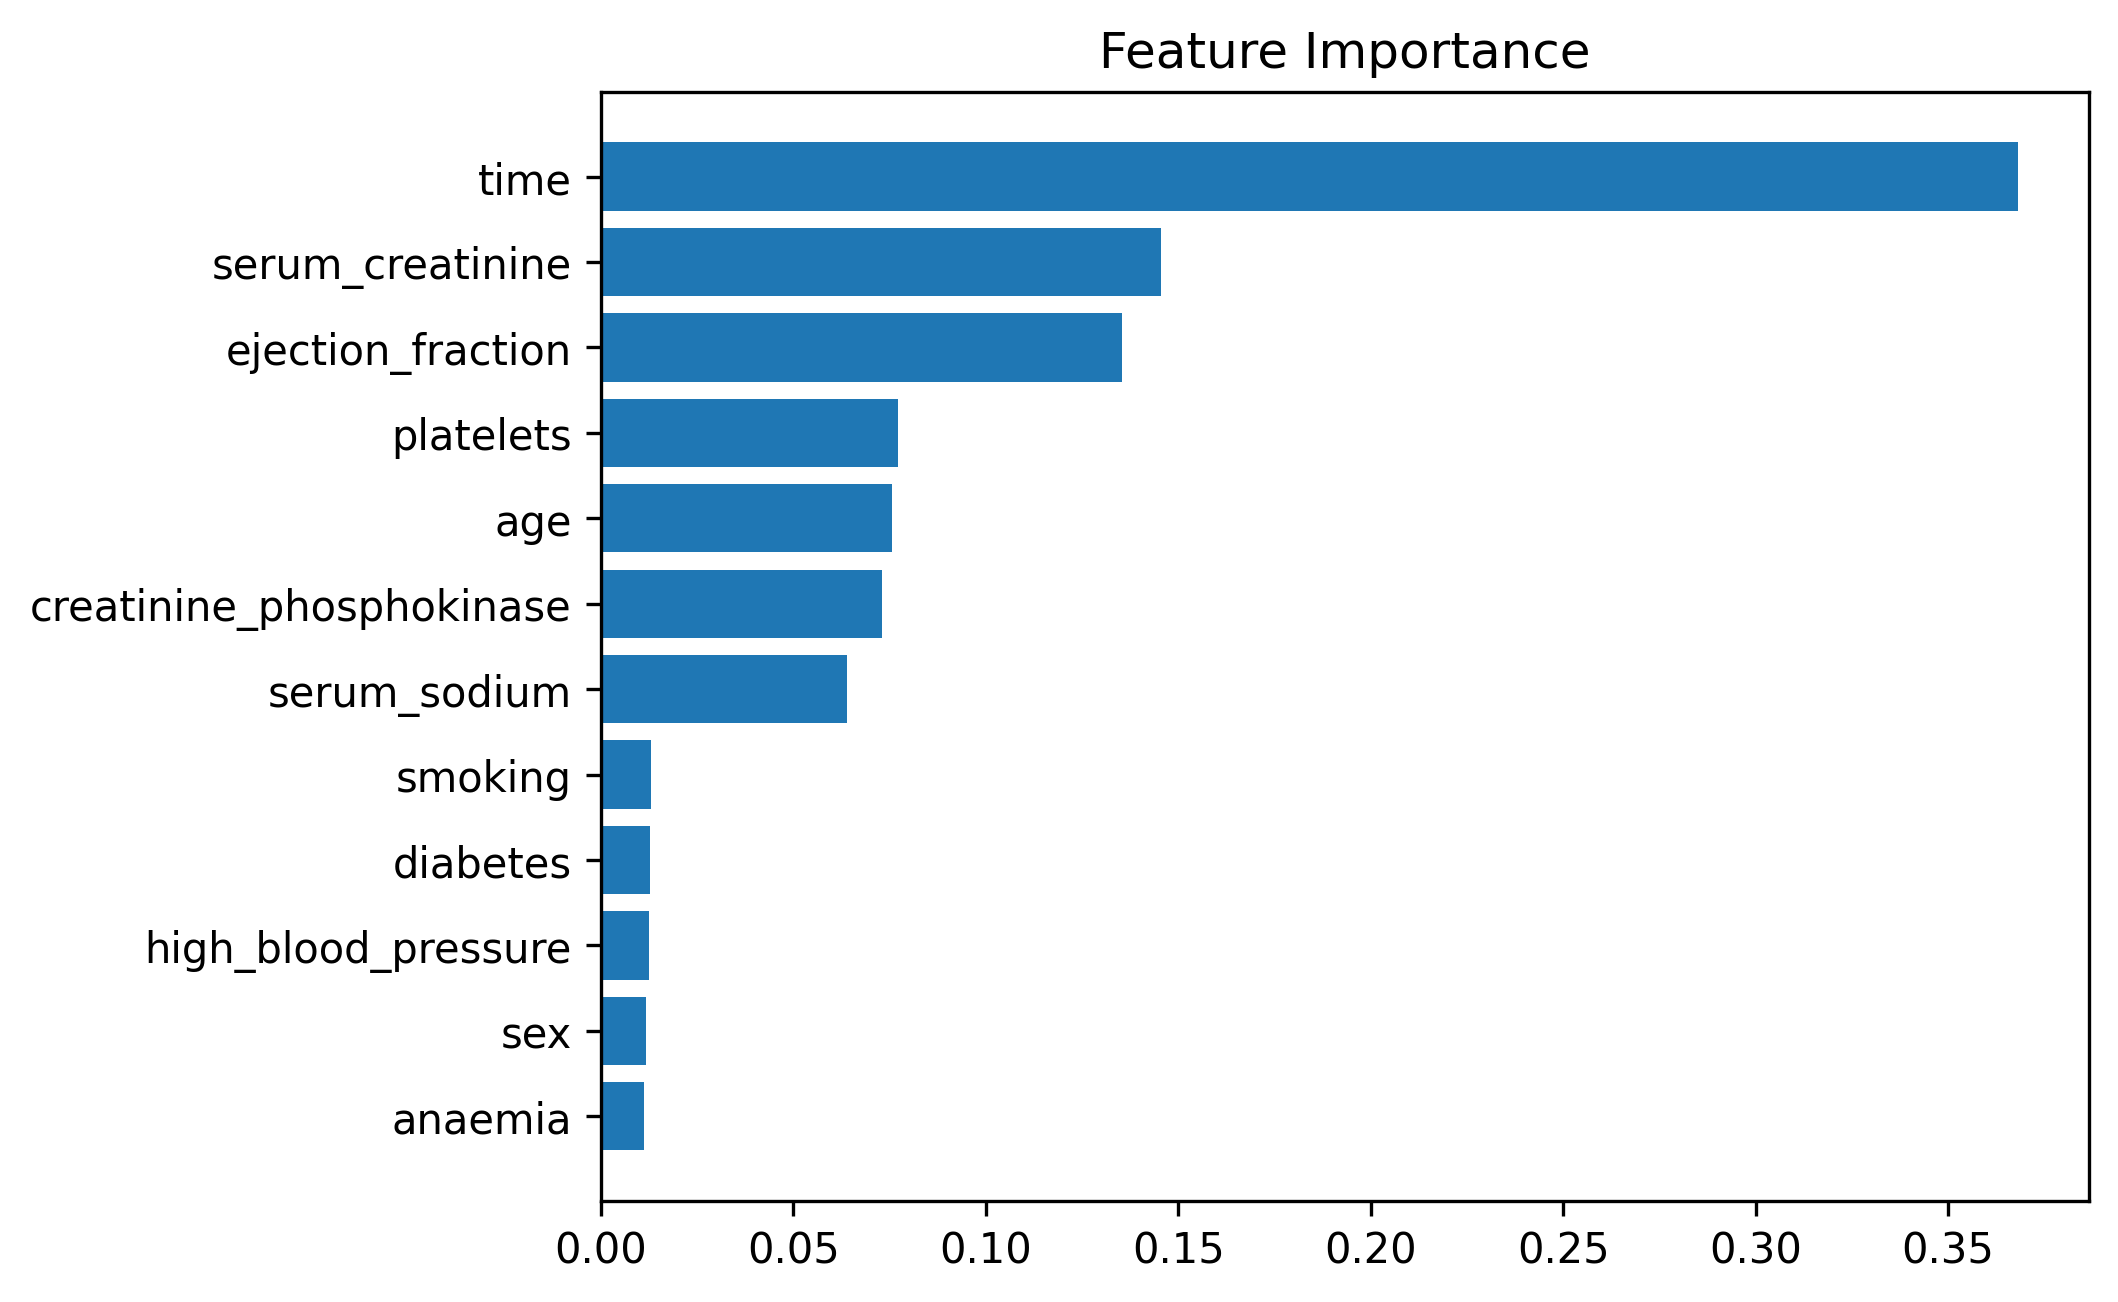
\includegraphics[width=0.6\textwidth]{../figures/feature_importance.png}
		\caption{Feature importance from Random Forest model}
	\end{figure}
	
	Feature importance analysis reveals that the most influential variable is ``time''. However, this variable represents follow-up duration rather than a physiological condition.
	
	This raises an important methodological concern: time may introduce information leakage, as longer follow-up inherently increases the probability of observing an event.
	
	After excluding this variable, serum creatinine and ejection fraction remain the most important clinically meaningful predictors.
	
	% ==================================================
	\section{Discussion}
	% ==================================================
	
	The integration of statistical analysis, visualization, and machine learning modeling provides a consistent interpretation of heart failure risk factors.
	
	Several key findings emerge:
	
	First, cardiac function (ejection fraction) and renal function (serum creatinine) are the strongest physiological predictors of mortality.
	
	Second, age plays a nonlinear but significant role in risk stratification.
	
	Third, class imbalance significantly affects model sensitivity, resulting in reduced recall.
	
	Finally, the presence of the ``time'' variable highlights the importance of careful feature selection in clinical machine learning applications.
	
	% ==================================================
	\section{Conclusion}
	% ==================================================
	
	This study demonstrates that Random Forest outperforms Logistic Regression in terms of AUC for heart failure survival prediction.
	
	More importantly, the analysis confirms that serum creatinine, ejection fraction, and age are key clinical risk factors.
	
	Future work should focus on handling class imbalance, improving recall, and removing potential leakage variables to enhance clinical reliability.
	
\end{document}